\documentclass[a4paper, twocolumn]{article}
\usepackage[pdftex, hidelinks,
            pdftitle={Machine Learning Report},
            pdfauthor={Erik Sven Vasconcelos Jansson},
            pdfsubject={Machine Learning Report},
            pdfkeywords={report}]{hyperref}

\usepackage{bm}
\usepackage[T1]{fontenc}
\usepackage[utf8]{inputenc}
\usepackage{algorithmic}
\usepackage{algorithm}
\usepackage{amsfonts}
\usepackage{booktabs}
\usepackage{amssymb}
\usepackage{courier}
\usepackage{booktabs}
\usepackage{graphicx}
\usepackage{listings}
\usepackage{mathtools}
\usepackage[capitalize, noabbrev]{cleveref}
\lstset{basicstyle=\footnotesize\ttfamily,
        breakatwhitespace = false,
        breaklines = true,
        keepspaces = true,
        language = C++,
        showspaces = false,
        showstringspaces = false,
        belowcaptionskip = \bigskipamount,
        framerule = 0.80pt,
        frame = tb,
        numbers = left,
        belowskip = \bigskipamount,
        escapeinside={<@}{@>}}

\title{Introduction to Machine Learning \\
       Individual Laboration Report --4--}
\author{{Erik Sven Vasconcelos Jansson} \\
        {\href{mailto:erija578@student.liu.se}
        {\texttt{erija578@student.liu.se}}} \\
        {Linköping University, \, Sweden}}

\begin{document}

    \pagenumbering{arabic}
    \maketitle % Titles...

    \section*{Assignment 1}

        We are given the data set \emph{State}, where observations regarding the \emph{metropolitan ratio} and the \emph{local public expenditure} for several \emph{states} exist. Plotting these against each other gives \cref{fig:state}. Notice that the data is quite spread out, and that there doesn't seem to be any easily visible pattern unfortunately.

        \begin{figure}[h!]
            \centering
            \caption{Metropolitan Ratio vs Expenditures (\$)}
            \label{fig:state}
            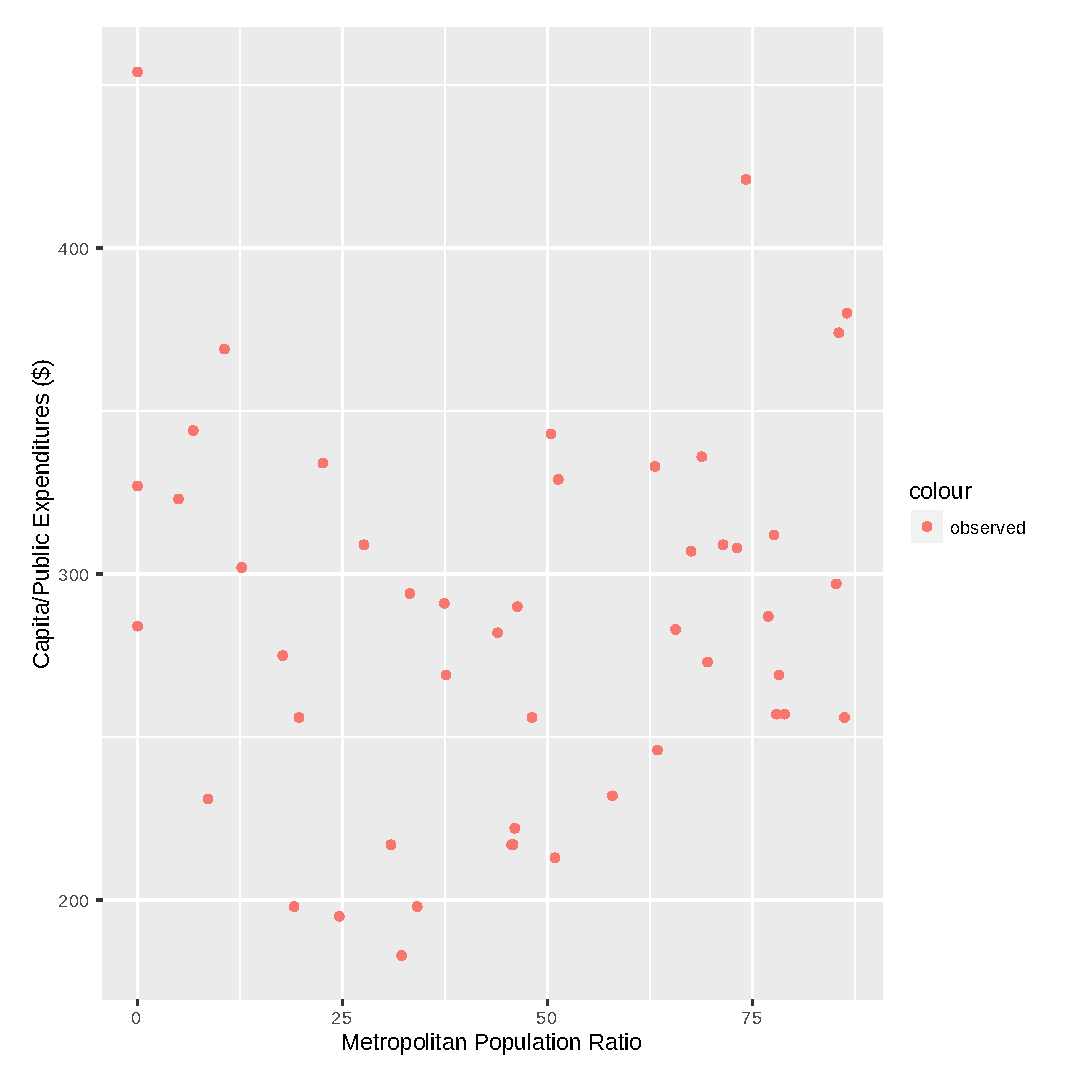
\includegraphics[width=0.5\textwidth]{share/state.eps}
        \end{figure}

        For this task we are recommended to use \emph{regression trees} as the \emph{predictor} for the above situation. We fit the model using all observations, and thereafter \emph{cross-validate} the model to find the optimal number of leaves for the \emph{decision tree}. See \cref{fig:tree}.

        \begin{figure}[h!]
            \centering
            \caption{Optimal Regression Tree Predictor}
            \label{fig:tree}
            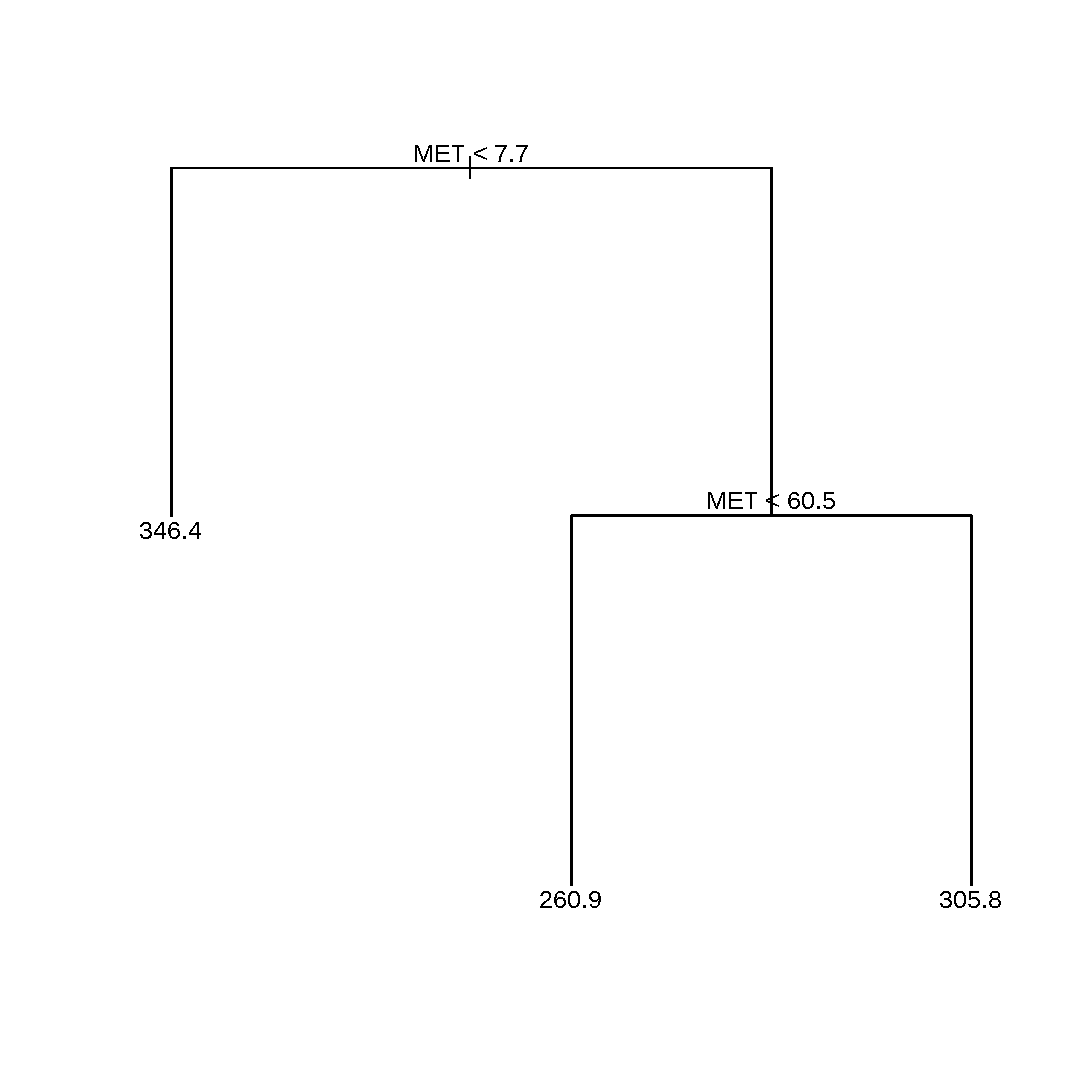
\includegraphics[width=0.5\textwidth]{share/tree.eps}
        \end{figure}

        Notice that \emph{three leaves} have been selected, therefore, the \emph{optimal regression tree} is found by \emph{pruning} the original tree and obtaining the above. This is done in \cref{lst:assignment1} under source lines \verb|20-30|.

        Thereafter, we predict the observed data using our optimal regression tree. Plotting these against the original observations gives \cref{fig:predicted_state}. Notice how the predictor has given estimates that are roughly the \emph{mean} of each ``bucket'' selected by the regression tree. Therefore, the selected model is not expected to perform very good since it does not account for the noise present in the model very well, but will predict some correctly, since it's around the mean.

        \begin{figure}[h!]
            \centering
            \caption{Regression Tree Predicted Expenditure}
            \label{fig:predicted_state}
            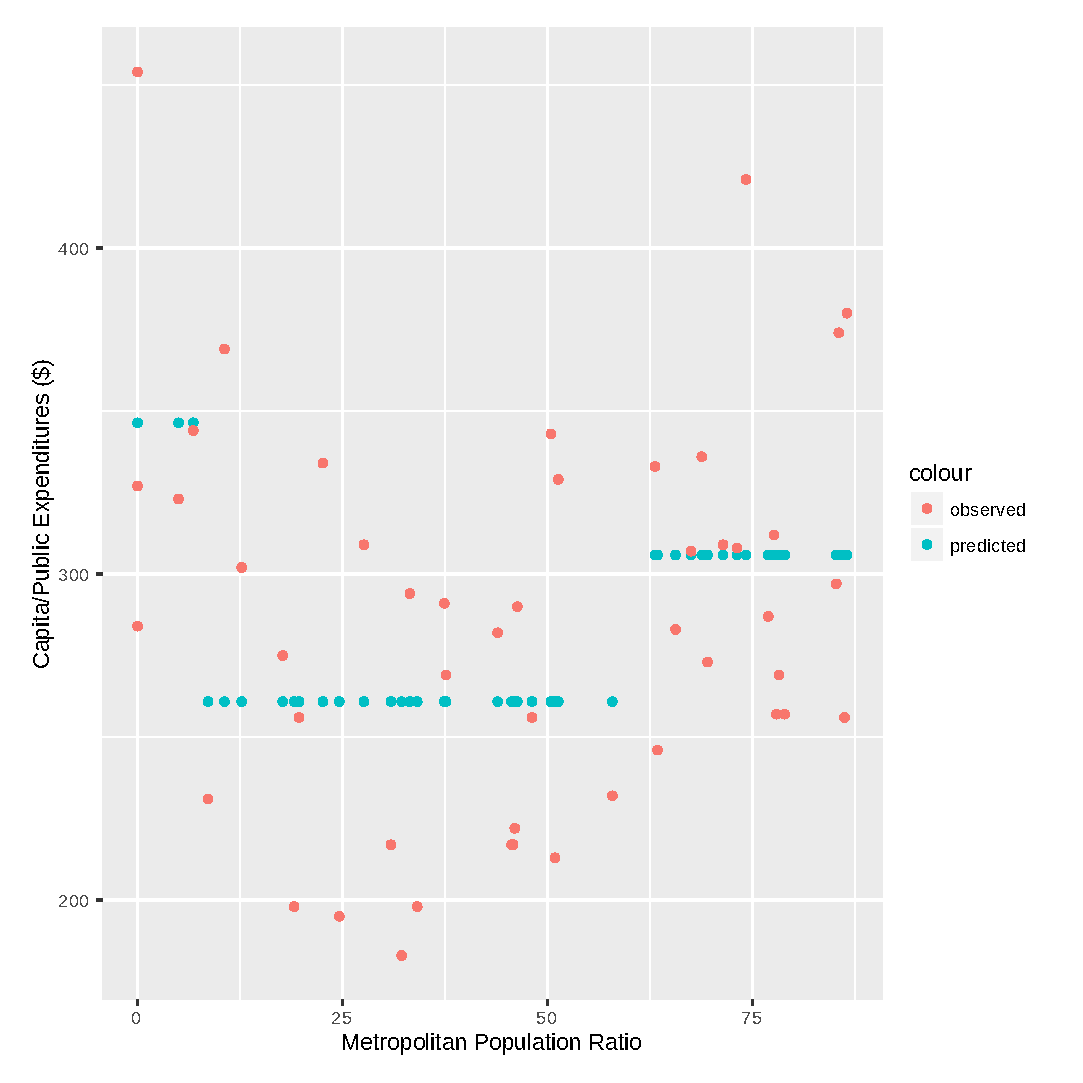
\includegraphics[width=0.5\textwidth]{share/predicted_state.eps}
        \end{figure}

        Finally, we plot the \emph{residuals} from the \emph{regression tree model}, which are basically the \emph{distance} between the \emph{observed responses} and the \emph{predicted responses}. See \cref{fig:histogram}, where we have plotted a histogram of the residuals. Notice that it \emph{doesn't} resemble a \emph{bell curve}, meaning the \emph{error isn't normally distributed}.

        \begin{figure}[h!]
            \centering
            \caption{Histogram of Prediction Residuals}
            \label{fig:histogram}
            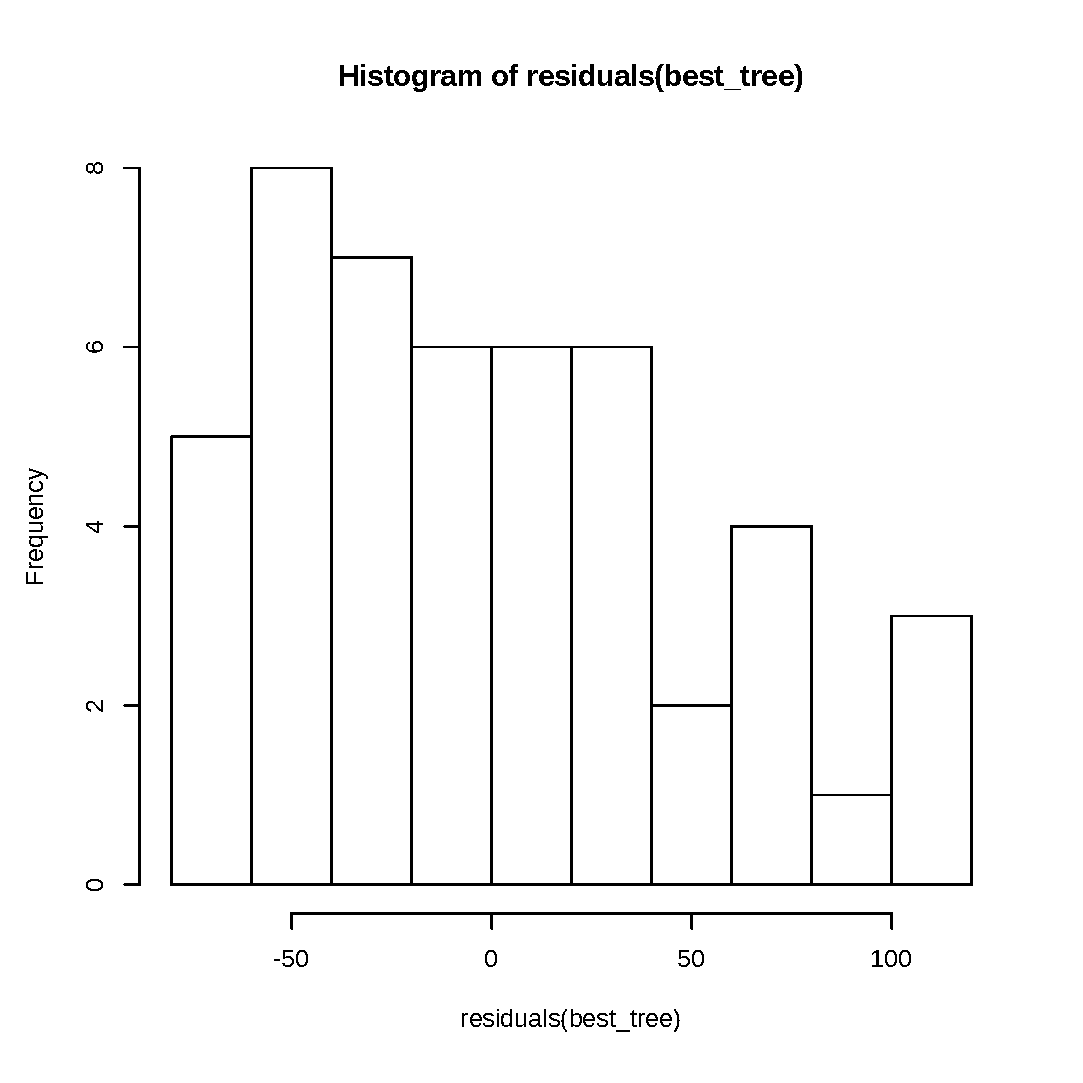
\includegraphics[width=0.5\textwidth]{share/histogram.eps}
        \end{figure}

        Since the chosen model doesn't seem particularly good, at least for these observations, we want to find \emph{more information} about our estimator. Using \emph{bootstrap} seems like a good idea. \emph{Bootstrapping} is used to \emph{estimate the properties} of an estimator by \emph{re-sampling} from a given \emph{approximated distribution}.

        Because we don't know the underlying distribution, we want to use \emph{non-parametric bootstrapping}. It works by \emph{re-sampling observations} with \emph{replacement}, the distribution is then calculated by using: \(\hat{f}(D_1), \hat{f}(D_2), ..., \hat{f}(D_B)\), where \(\hat{f}\) is our estimator. We use the \verb|boot| function in \emph{R}, re-sampling 1024 times. See \cref{lst:assignment1} lines \verb|49-64| for the algorithm.

        \begin{figure}[h!]
            \centering
            \caption{Non-Parametric Bootstrap C.B.}
            \label{fig:npbands}
            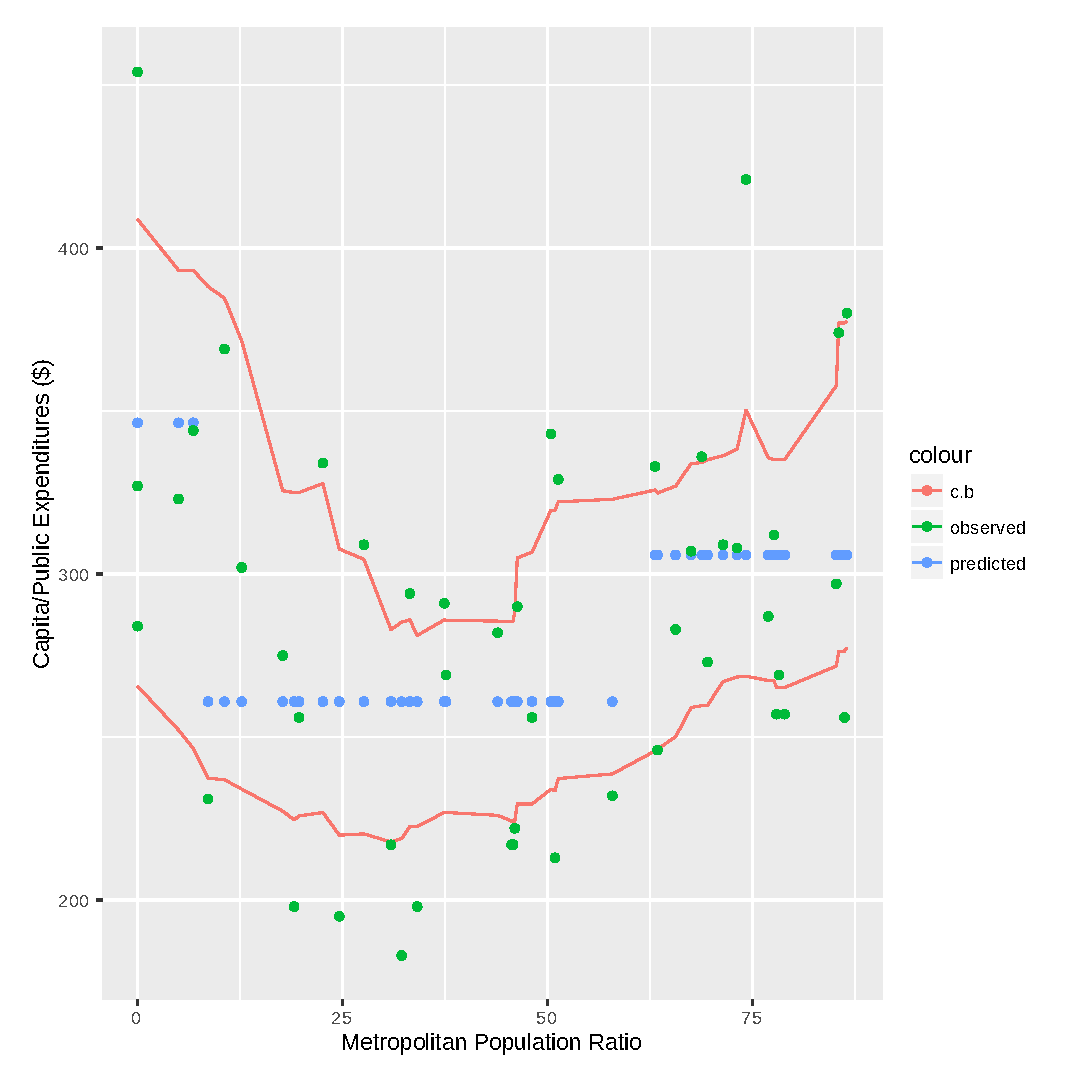
\includegraphics[width=0.5\textwidth]{share/npbands.eps}
        \end{figure}

        According to \cref{fig:npbands} which displays the plot of the \emph{confidence bands} of our estimator, several of our observations fall outside the \(95 \%\) confidence level, which means that our estimator isn't good at all. The curve also seems to be quite bumpy, because the predictor only jumps between the three leaves.

        Now, we are given a precondition: \(Y \sim \mathcal{N}(\mu_i, \sigma^2)\) which means the \emph{target} is now \emph{normally distributed}. In light of this, we can use \emph{parametric bootstrapping}, since the distribution has now been assumed to be known. It functions by re-sampling from the given distribution, which is different from before since we were only taking samples from the original data set, while we now generate entirely new, fresh, samples.

        By doing this in \cref{lst:assignment1} under lines \verb|82-114| we retrieve both the \emph{confidence} and \emph{prediction bands}. Both of these bands are plotted in \cref{fig:pbands} below.

        \begin{figure}[h!]
            \centering
            \caption{Parametric Bootstrap C.B. + P.B.}
            \label{fig:pbands}
            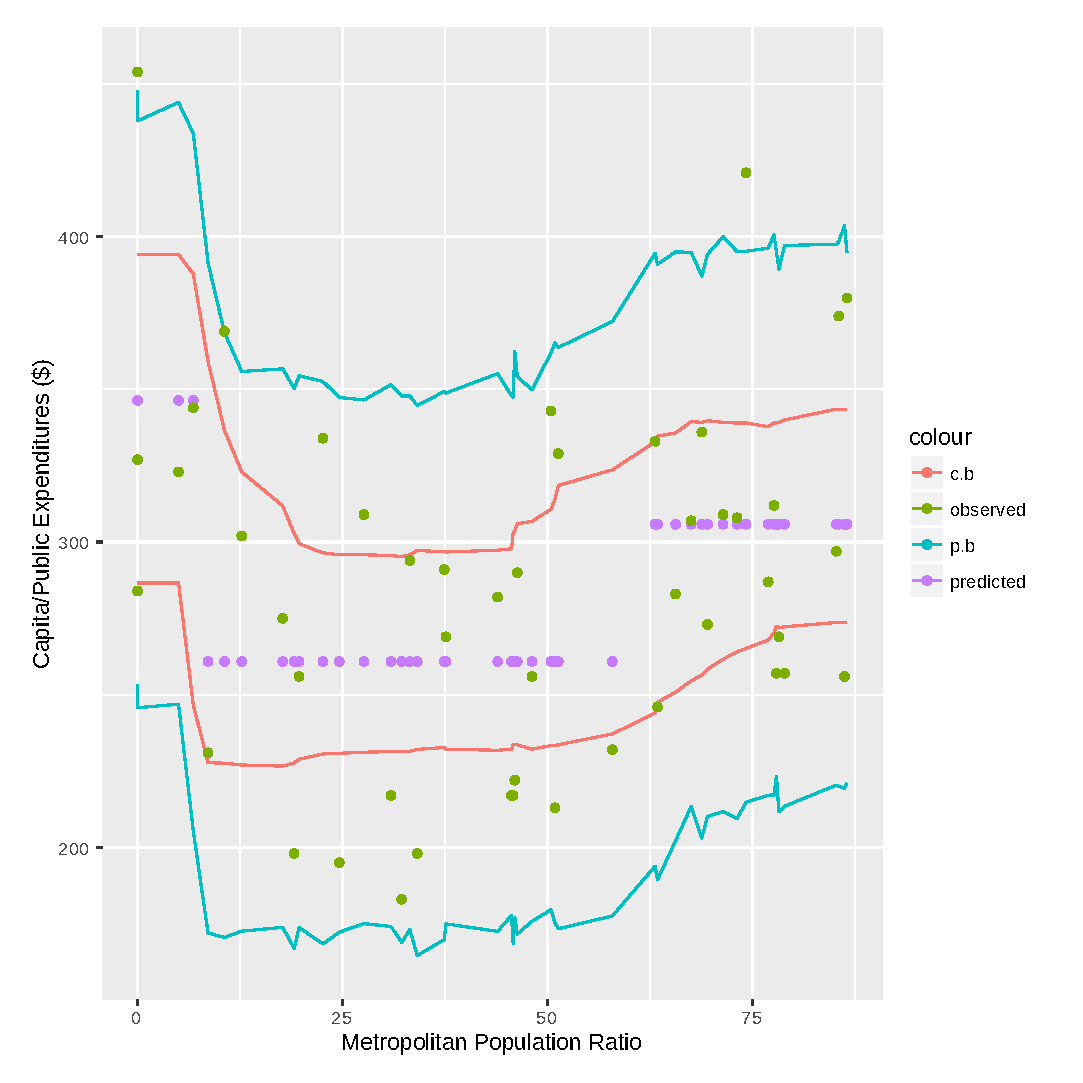
\includegraphics[width=0.5\textwidth]{share/pbands.eps}
        \end{figure}

        Notice, that the \emph{prediction band} covers most of the observations, as opposed to the \emph{confidence band}. \emph{Prediction bands} account for the \emph{noise} in the data. It seems reasonable that around \(5 \%\) of the observations fall outside the \emph{prediction band}, since we are targeting a \(95 \%\) level of confidence (or by \(\alpha = 5 \%\)). In this case, the model which we have predicted seems reasonable, since most predictions are right. \emph{However}, this is probably not true, since \cref{fig:histogram} shows a distribution that is most likely not normal, therefore \emph{non-parametric bootstrapping} seems more accurate in this particular case (also by intuition).

    \section*{Assignment 2}

        Here, we are given a data set containing measures of \emph{near-infrared spectra} and their \emph{viscosity level} for a collection of \emph{diesel fuels}. There are a lot of \emph{features}.

        \emph{Principal Component Analysis (PCA henceforth)} is a \emph{dimensionality reduction} technique, where the goal is to find a set of \emph{principal components} where the given \emph{observations} are might to be correlated. Our task is to find the \emph{principal components} of the given data set accounting for \(99 \%\) of the variance.

        By using the built-in \verb|prcomp| function, we apply \emph{PCA} in \cref{lst:assignment2} under lines \verb|7-17|. Afterwards in \cref{fig:screeplot} we produce a \emph{scree plot}, which tells us that \emph{two features} seem to account for all of the variance. More accurately, a bit above \(99 \%\) of the variance...

        \begin{figure}[h!]
            \centering
            \caption{Scree Plot for PCA}
            \label{fig:screeplot}
            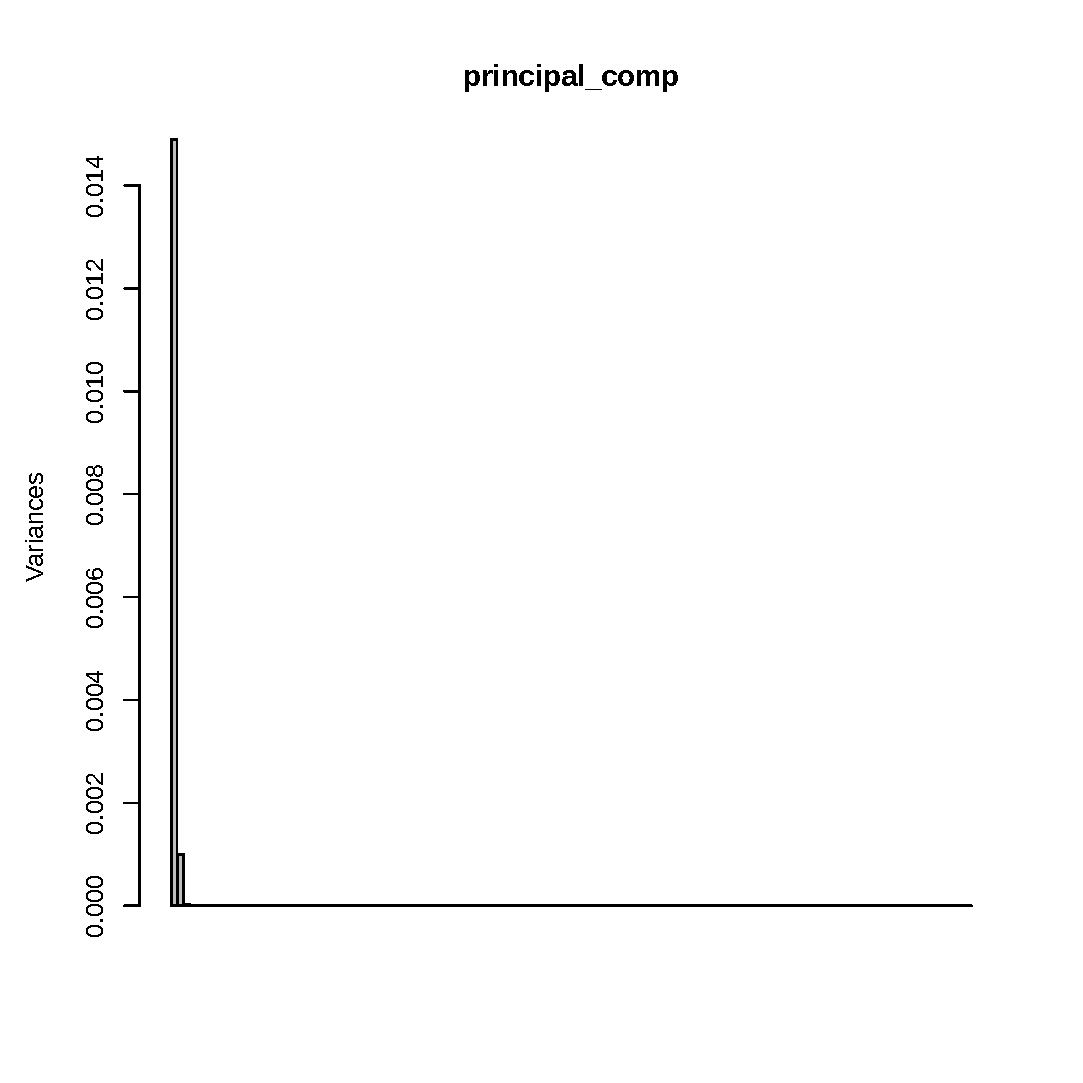
\includegraphics[width=0.4\textwidth]{share/screeplot.eps}
        \end{figure}

        Additionally, the chosen features \emph{X750} and \emph{X752} are plotted against each other, giving the \cref{fig:score}. Notice that there are a couple of outliers in \([1.0, 1.5]\) which can be classified as being \emph{unusual diesel fuels}.

        \begin{figure}[h!]
            \centering
            \caption{Score for PC1 and PC2}
            \label{fig:score}
            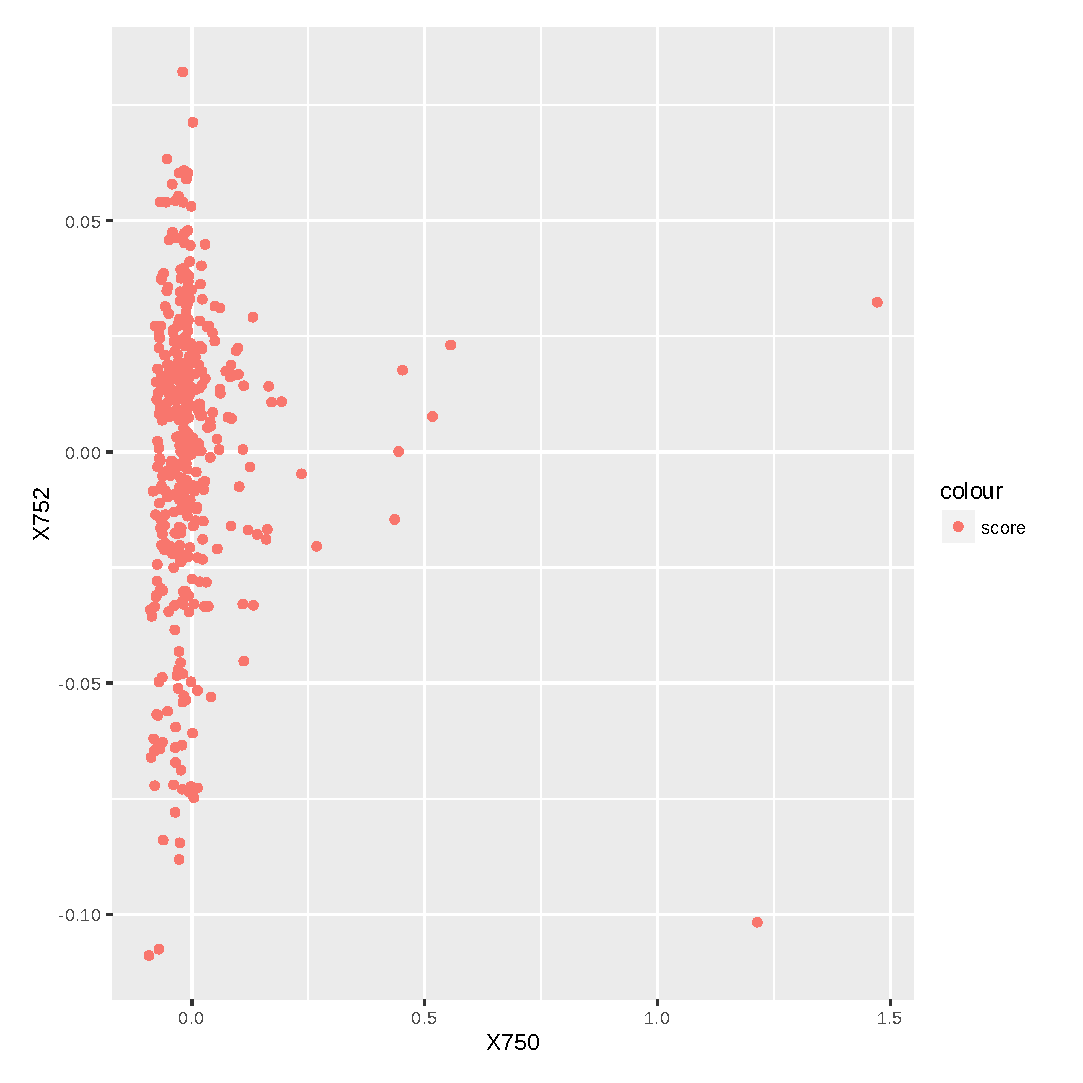
\includegraphics[width=0.5\textwidth]{share/score.eps}
        \end{figure}

        Plotting the so called \emph{loadings} of these principal components gives \cref{fig:pcloadings}. A high \emph{loading} implies that there is a \emph{strong correlation} for a given feature.

        \begin{figure}[h!]
            \centering
            \caption{Trace Plot of PCA Loadings}
            \label{fig:pcloadings}
            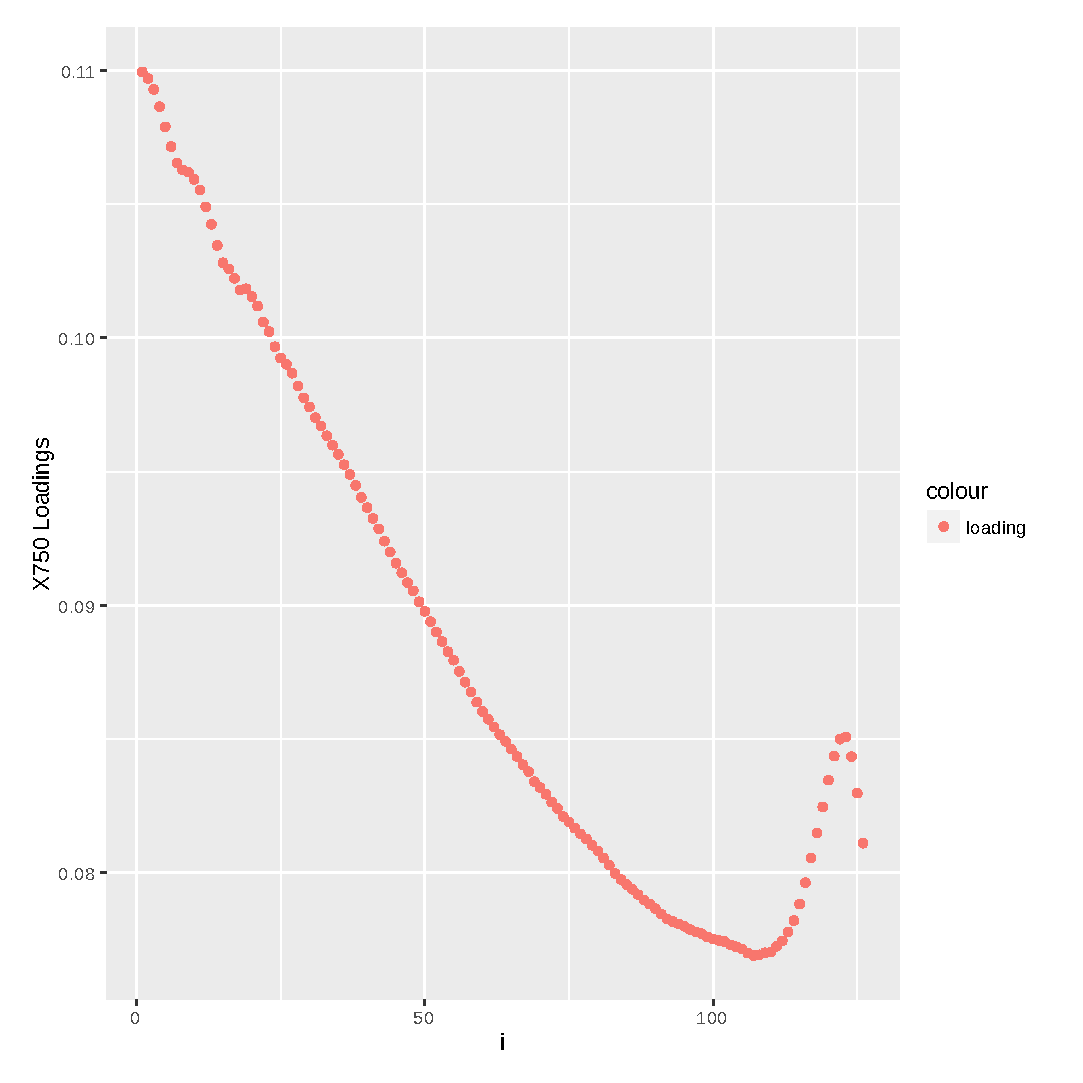
\includegraphics[width=0.5\textwidth]{share/x750loadings.eps}
            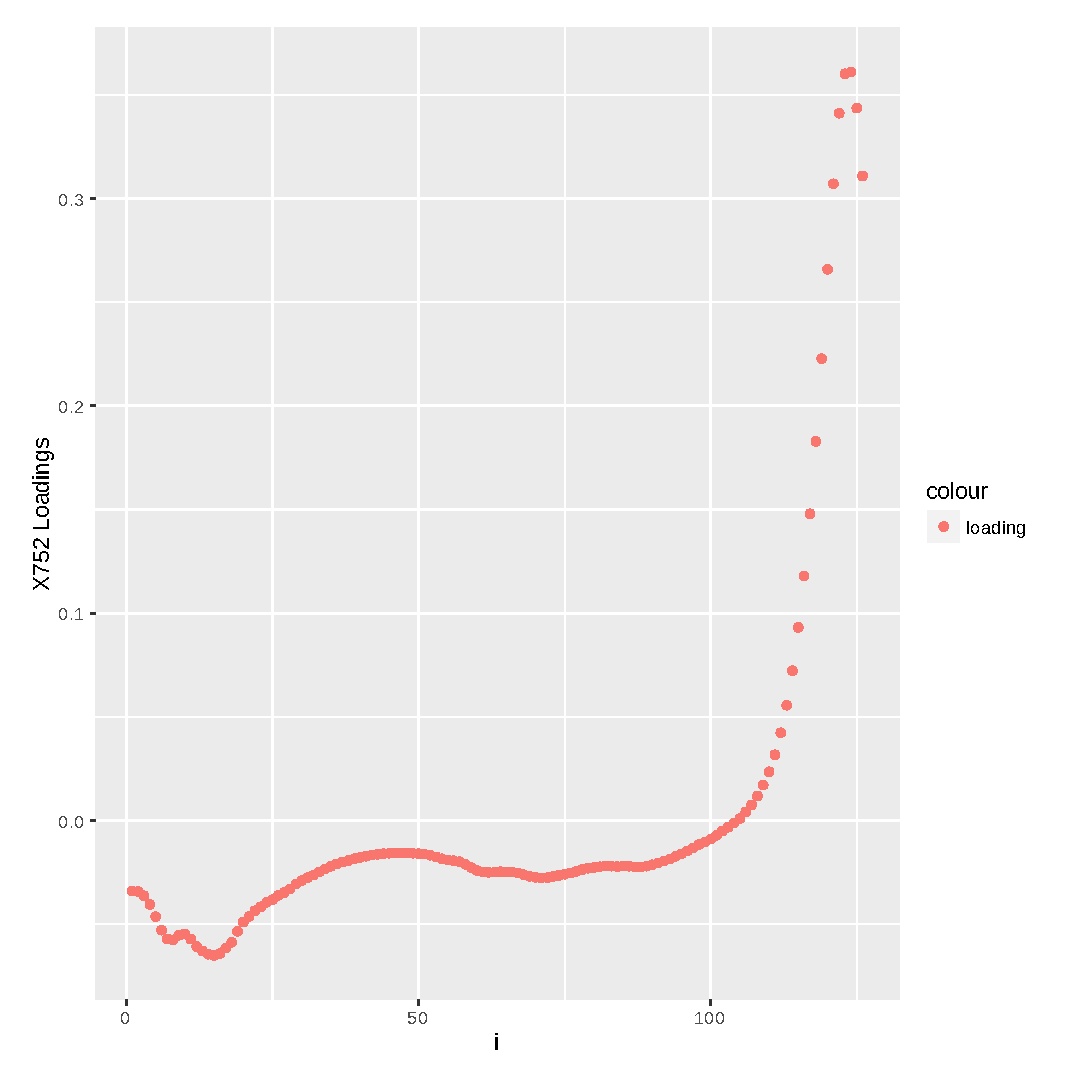
\includegraphics[width=0.5\textwidth]{share/x752loadings.eps}
        \end{figure}

        Notice that both PC1 and PC2 seem to have a correlated feature(s) that spike in loading amount, while the rest seem to less significant in comparison. This might be a good candidate for a third principal component if we required to have higher variance.

        Now we apply \emph{Independent Component Analysis} instead, which assumes the given components are statistically independent. We do this in \cref{lst:assignment2} under lines \verb|45-68|, and produce the \emph{trace plot} for these in \cref{fig:icaloadings}. The contents of these plots are similar to those in \cref{fig:pcloadings}, which are \emph{loadings}, but are inverted, since we are measuring \emph{independence} instead of \emph{correlation}, the opposite PCA measure. Finally, we plot the score(s) of these in \cref{fig:scores}.

        \begin{figure}[h!]
            \centering
            \caption{Trace Plot of ICA Loadings}
            \label{fig:icaloadings}
            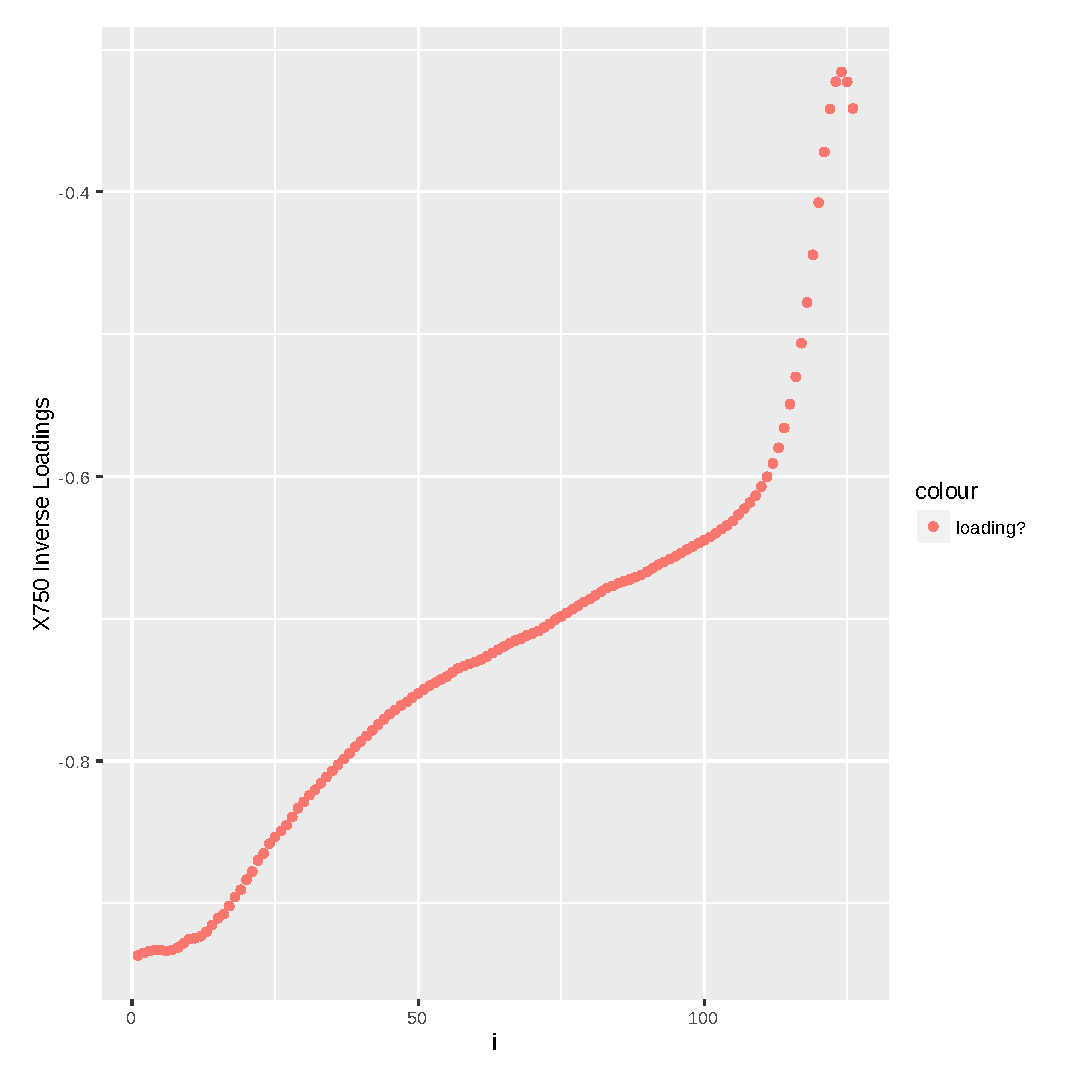
\includegraphics[width=0.5\textwidth]{share/x750traceplot.eps}
            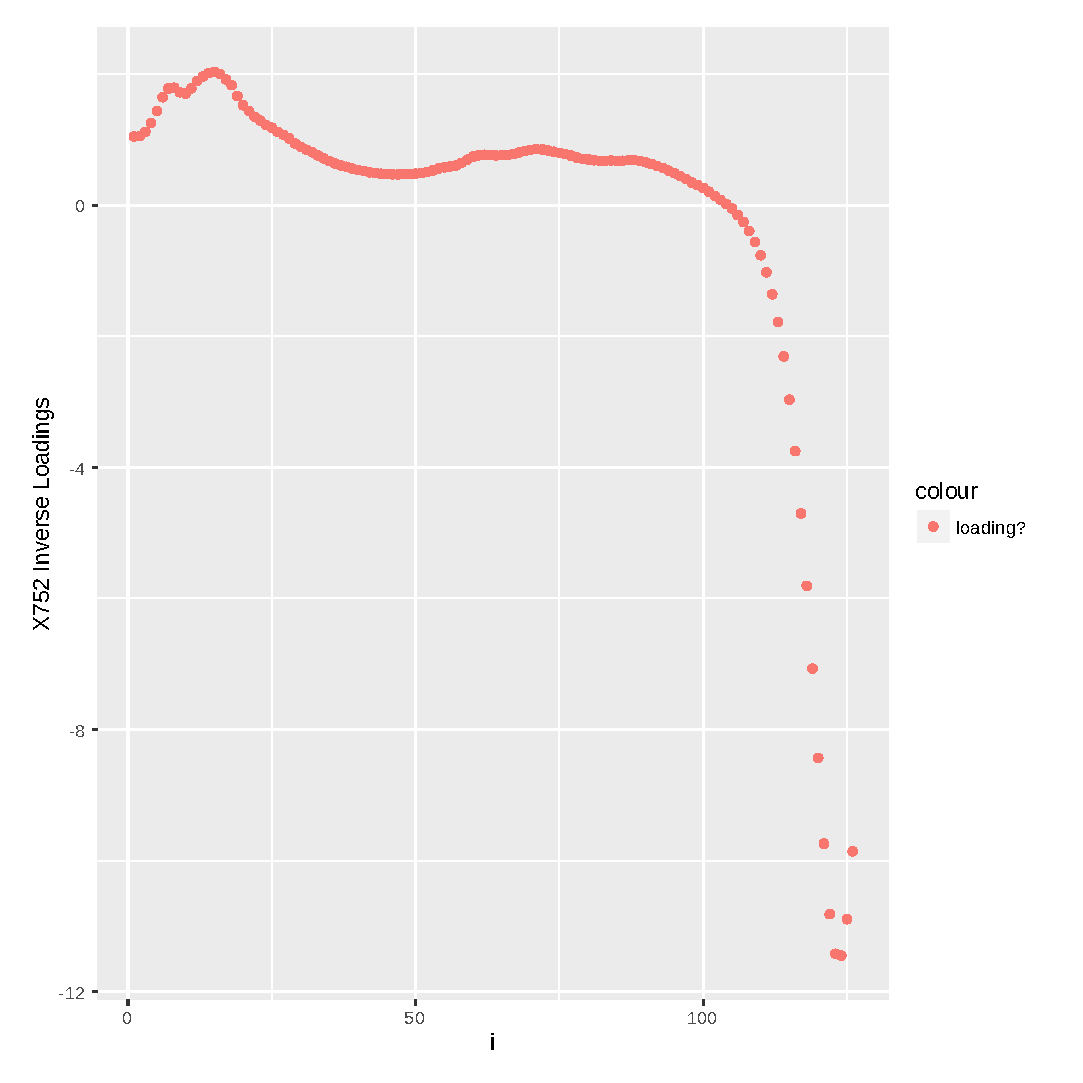
\includegraphics[width=0.5\textwidth]{share/x752traceplot.eps}
        \end{figure}

        Notice that the direction of the score has been swapped, the underlying reason for this is similar to those previously mentioned regarding loadings. It's interesting to note that the units are different.


        \begin{figure}[h!]
            \centering
            \caption{Score for PCA and ICA}
            \label{fig:scores}
            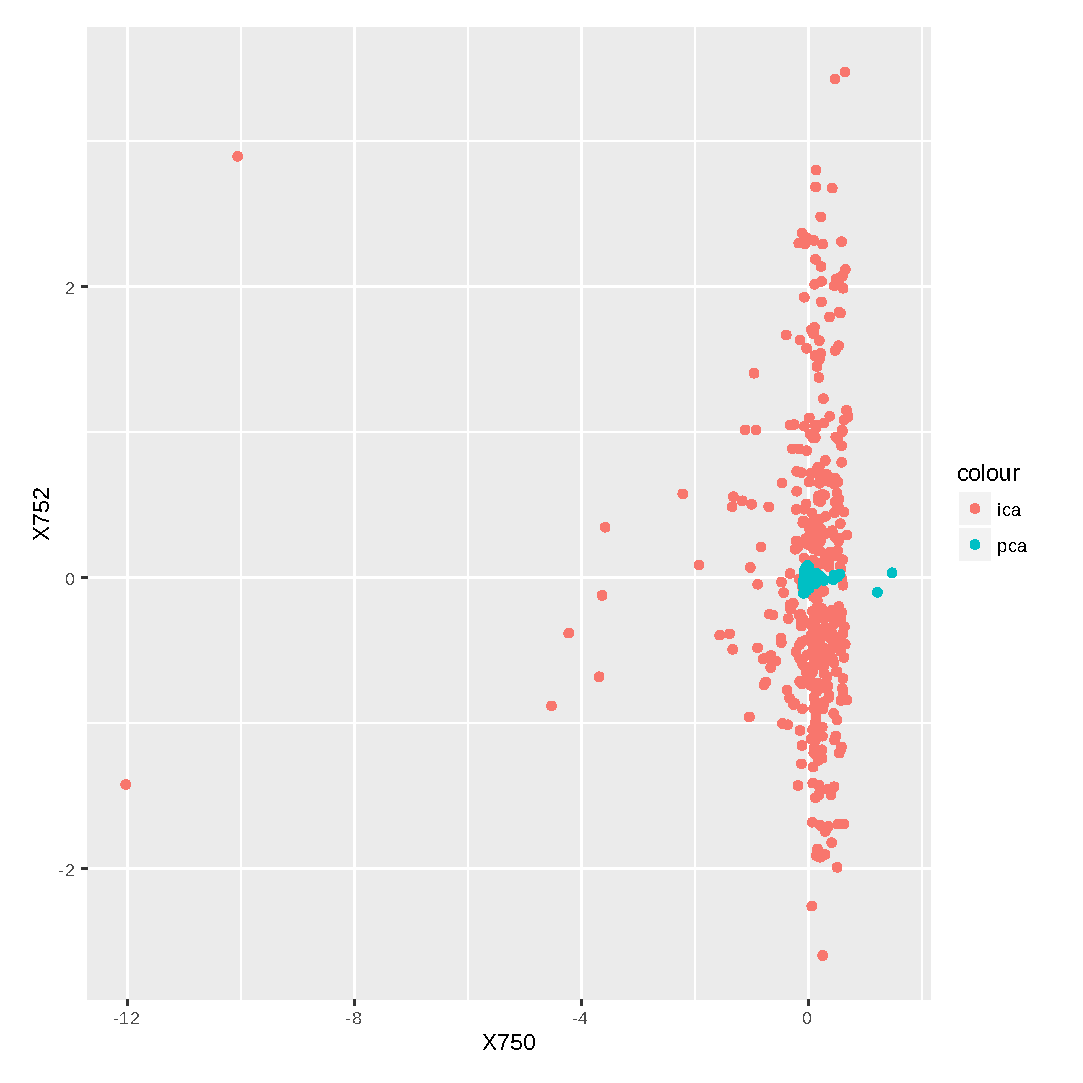
\includegraphics[width=0.5\textwidth]{share/icascore.eps}
        \end{figure}

        Finally, we apply \emph{cross-validation} in \cref{fig:scores}, and note that the ranges of \([10, 18]\) p.c.\ components produces least \emph{MSE}, in relation to the p.c.\ amount.

        \begin{figure}[h!]
            \centering
            \caption{Cross-Validation for PCA}
            \label{fig:pcacv}
            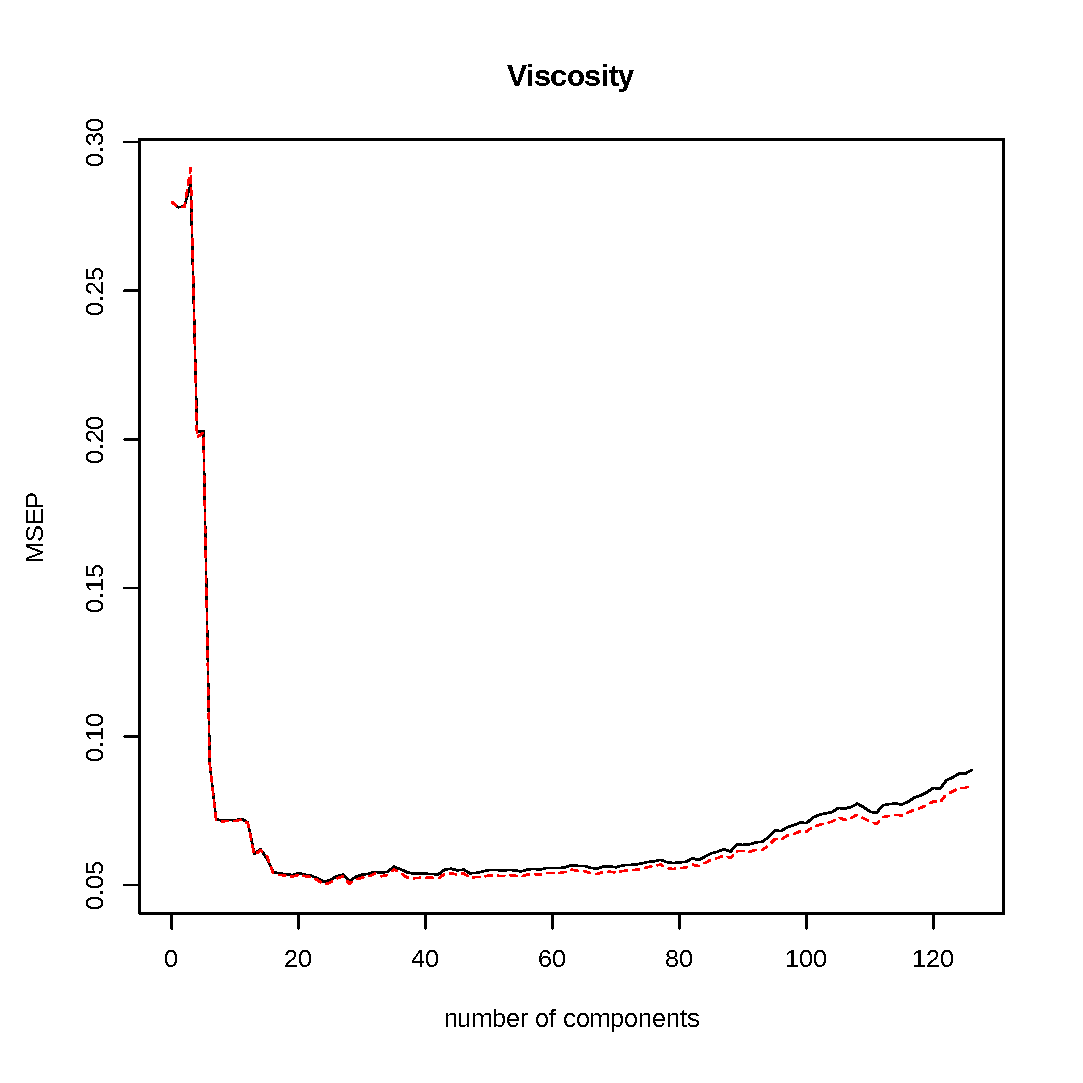
\includegraphics[width=0.45\textwidth]{share/pcacv.eps}
        \end{figure}

    \nocite{*}
    \bibliographystyle{alpha}
    \bibliography{report}

    \onecolumn \appendix
    \section*{Appendix}

    \lstinputlisting[caption={Script for Assignment 1 on Bootstrapping Regression Tree Model},label={lst:assignment1}]{../share/assignment1.r}
    \lstinputlisting[caption={Script for Assignment 2 on Principal/Individual Component Analysis},label={lst:assignment2}]{../share/assignment2.r}

\end{document}
